\chapter{}\label{chp:2}
In order to design a chip layout including a certain number of regular components $cr$ and a certain number of power components $cp$, several constraints are applicable in the general case, these will be discussed first. Furthermore some constraints are specific to the version of the problem being solved, these will be discussed after that.

First of all it needs to be specified that all components need to fit on the chip. This is equivalent to stating that the origin of each component should be larger than or equal to zero in both the horizontal and the vertical direction and stating that the origin plus the size of each component should be smaller than or equal to the size of the chip, again in both the horizontal and the vertical direction. This constraint is formalized by \Cref{eqn:2_allfit}, where $W$ and $H$ are parameters of the specific problem which will be specified in \Cref{eqn:2_whd}.
\begin{equation}
  \label{eqn:2_allfit}
  \begin{aligned}
    \bigwedge_{i = 0}^{cp + cr}
      &(X_{i} \geq 0) \wedge
       (Y_{i} \geq 0) \wedge \\
      &(X_{i} + W_{i} \leq W) \wedge
       (Y_{i} + H_{i} \leq H)
     \end{aligned}
\end{equation}

Next it must be specified that no components may overlap. This is equivalent to stating that the origin of component $i$ is larger than or equal to the origin plus the size of component $j$ or the other way around for all distinct pairs of components $i$ and $j$. This requirement is exactly captured by \Cref{eqn:2_overlap}.
\begin{equation}
  \label{eqn:2_overlap}
  \begin{aligned}
    \bigwedge_{i = 0}^{cp + cr}
      \bigwedge_{j = 0, i \neq j}^{cp + cr}
        &(X_{i} \geq X_{j} + W_{j}) \vee
         (Y_{i} \geq Y_{j} + H_{j}) \vee \\
        &(X_{j} \geq X_{i} + W_{i}) \vee
         (Y_{j} \geq Y_{i} + H_{i})
  \end{aligned}
\end{equation}

Furthermore it needs to be specified that all regular components are connected to a power component. This is equivalent to stating that at least one of the edges of the regular component $i$ shares a point with any of the edges of any of the power components $0 \leq j < cp$, for all regular components. Stating this can be expressed by asserting that either pair of vertical edges must be at the same horizontal position while the components overlap in the vertical direction, or either pair of horizontal edges must be at the same vertical position while the components overlap in the horizontal direction. Since the components cannot overlap due to \Cref{eqn:2_overlap}, only the right edge of the regular component has to be compared to the left edge of the power component and vice versa. Similarly only the top edge of the regular component has to be compared to the bottom edge of the power component and vice versa. The formalized version of this constraint is shown in \Cref{eqn:2_power}.
\begin{equation}
  \label{eqn:2_power}
  \begin{aligned}
    \bigwedge_{i = cp}^{cp + cr}
      \bigvee_{j = 0}^{cp - 1}
        \Bigg(
          \Big(
           &(X_{i} = X_{j} + W_{j}) \vee
            (X_{j} = X_{i} + W_{i})
          \Big) \wedge \\
         &(Y_{i} \leq Y_{j} + H_{j}) \wedge
          (Y_{j} \leq Y_{i} + H_{i})
        \Bigg) \vee \\
        \Bigg(
          \Big(
           &(Y_{i} = Y_{j} + H_{j}) \vee
            (Y_{j} = Y_{i} + H_{i})
          \Big) \wedge \\
         &(X_{i} \leq X_{j} + W_{j}) \wedge
          (X_{j} \leq X_{i} + W_{i})
        \Bigg)
    \end{aligned}
\end{equation}

The last general constraint that needs to be specified is that there should exist a certain distance between the centers of all of the power components in the horizontal or the vertical direction. This constraint is detailed in \Cref{eqn:2_dist}, which simply states that the center of component $i$ minus the center of component $j$ should be larger than or equal to a certain distance $D$ in either direction. The distance $D$ is specified in \Cref{eqn:2_whd}.
\begin{equation}
  \label{eqn:2_dist}
  \begin{aligned}
    \bigvee_{i = 0}^{cp - 1}
      \bigvee_{j = 0, i \neq j}^{cp - 1}
        &\Big((X_{i} + \frac{1}{2}W_{i}) - (X_{j} + \frac{1}{2}W_{j}) \geq D\Big) \vee \\
        &\Big((Y_{i} + \frac{1}{2}H_{i}) - (Y_{j} + \frac{1}{2}H_{j}) \geq D\Big)
  \end{aligned}
\end{equation}

Finally two constraints exist that are specific to the instance of the problem being solved, the first of which states the width $W$ and height $H$ of the chip and the distance $D$ between the power components. This constraint is shown in \Cref{eqn:2_whd}.
\begin{equation}
  \label{eqn:2_whd}
  W = 30 \wedge H = 30 \wedge D = 18
\end{equation}

Lastly it is necessary to specify the widths and heights of each component. In this constraint the possibility to rotate all components $90\degree$ is incorporated by also allowing the width and height to be swapped for each component. This constraint for the specified problem is shown in \Cref{eqn:2_sizes}. Since for this problem $cp = 2$ and $cr = 10$, the components with subscript $0$ and $1$ are the power components, while all other components are regular components.
\newcommand{\IIsize}[3]{
  &\Big(
    (W_{#1} = #2 \wedge H_{#1} = #3) \vee
    (H_{#1} = #2 \wedge W_{#1} = #3)
  \Big)
}
\begin{equation}
  \label{eqn:2_sizes}
  \begin{aligned}
    \IIsize{0} {4} {3}  \wedge \\
    \IIsize{1} {4} {3}  \wedge \\
    \IIsize{2} {4} {5}  \wedge \\
    \IIsize{3} {4} {6}  \wedge \\
    \IIsize{4} {5} {20} \wedge \\
    \IIsize{5} {6} {9}  \wedge \\
    \IIsize{6} {6} {10} \wedge \\
    \IIsize{7} {6} {11} \wedge \\
    \IIsize{8} {7} {8}  \wedge \\
    \IIsize{9} {7} {12} \wedge \\
    \IIsize{10}{10}{10} \wedge \\
    \IIsize{11}{10}{20}
  \end{aligned}
\end{equation}

A Python script to generate the SMT-LIB v2 file containing the conjunction of all requirements is written and the contents are presented in \Cref{app:2_gen.py}. The requirements file generated by this script for the specific problem can be found in \Cref{app:2_req.smt}. Running the Z3 solver on this file produces an output which can be interpreted by another python script that generates an image for the layout determined from the requirements, if they are satisfiable. This script can be found in \Cref{app:2_draw.py}, it should be noted that this script is only able to interpret results in the Integer domain, since results in the Real domain can contain output such as \texttt{(define-fun X3 () Real (/ 47.0 2.0))} which this script is not designed to interpret.

For $D=18$ a solution is found in the Integer domain, and therefore also in the Real domain. The result for the Integer domain is shown visually in \Cref{fig:2_result}. For the cases where $D = 20$ or $D = 22$ no solution is found in the Real domain or in the Integer domain. In these two cases the requirements are unsatisfiable.
\begin{figure}[!ht]
  \centering
  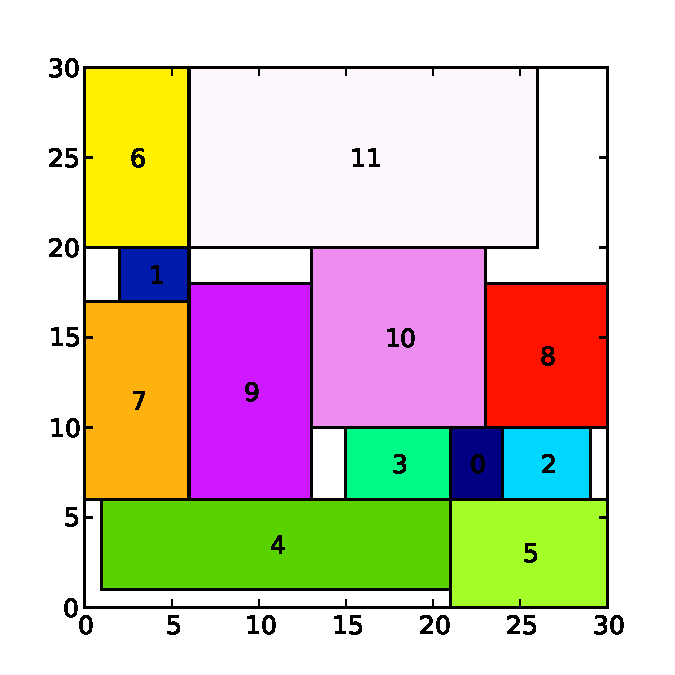
\includegraphics[width=\columnwidth]{2/chip_layout.pdf}
  \caption{The solution found for the specific version of the problem in the Integer domain}
  \label{fig:2_result}
\end{figure}
